\subsection{Physiological Dangers}
Characters might find themselves without food, water, or sleep and with no means to obtain them.

Characters who have taken nonlethal damage from lack of food, water, or sleep, are fatigued. Nonlethal damage from dehydration, starvation, or sleep deprivation, cannot be recovered until the character gets food, water, or sleep, as needed---not even magic that restores hit points heals this damage.

\begin{figure}[t!]
\centering
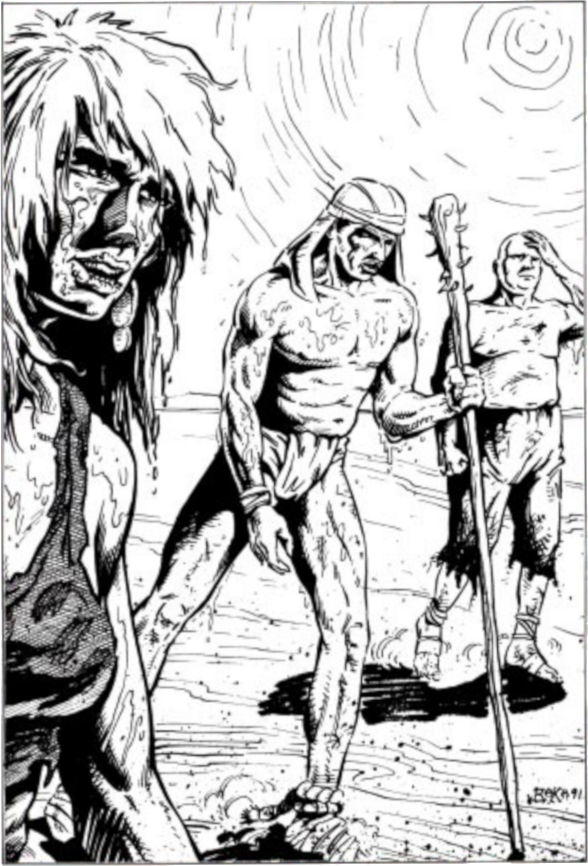
\includegraphics[width=\columnwidth]{images/dehydration.png}
\WOTC
\end{figure}

\subsubsection{Dehydration}
While in a temperate climate a character must consume 3 liters of water per day to avoid dehydration, the Tablelands are not so gentle.

In particularly hot environments (very hot or worse), characters need double the normal amount. The amount of water required to avoid dehydration increases by 3 liters per temperature band higher than very hot (so 6 liters in severe heat, 9 liters in extreme heat, and so on). If you are using \tabref{Temperature Over a Day}, then \tabref{Water Per Day} indicates how many liters are needed during a typical day for all character sizes.

\Table{Water Per Day}{p{13mm}RRRR}{
& \multicolumn{4}{c}{\tableheader Weather (Temperature, Wind)}\\
\cmidrule[.5pt]{2-5}
  \tableheader Character Size
& \tableheader Normal, Calm
& \tableheader Normal, Strong
& \tableheader Hot, Calm
& \tableheader Hot, Strong \\
Small  & 2 liters &  2 liters &  3 liters &  4 liters \\
Medium & 4 liters &  5 liters &  6 liters &  8 liters \\
Large  & 8 liters & 10 liters & 12 liters & 16 liters \\
}

A creature can go without water for a number of hours equal to 24 + its Constitution score (mul characters can go double that number). After this time, the creature must make a successful Constitution check each hour (DC 10, +1 for each previous check) or take 1d6 points of nonlethal damage. In particularly hot environments (very hot or worse), the time a creature can go without water before making Constitution checks is reduced. Each hour counts as one more hour per temperature band higher than very hot (so 2 hours in severe heat, 3 hours in extreme heat, and so on). See \tabref{Effective Hours Without Water} for reference of how many ``water hours'' are spend during each type of day. 

\Table{Effective Hours Without Water}{y{28mm}RRRR}{
& \multicolumn{4}{c}{\tableheader Weather (Temperature, Wind)}\\
\cmidrule[.5pt]{2-5}
  \tableheader Protection
& \tableheader Normal, Calm
& \tableheader Normal, Strong
& \tableheader Hot, Calm
& \tableheader Hot, Strong \\
No protection           & 32 hours & 43 hours & 46 hours & 70 hours \\
Desert outfit           & 24 hours & 32 hours & 29 hours & 46 hours \\
Shelter                 & 24 hours & 24 hours & 24 hours & 29 hours \\
Desert outfit + shelter & 24 hours & 24 hours & 24 hours & 24 hours \\
}

\textbf{Dehydrated:} Characters who have taken nonlethal damage from lack of water are considered dehydrated and become fatigued. In addition, if a dehydrated character would take nonlethal damage from hot conditions, that damage instead becomes lethal damage.

A character who falls unconscious from nonlethal damage due to thirst begins to take the same amount of lethal damage instead. Damage from thirst, whether lethal or nonlethal, cannot be recovered until the character has been treated; not even magic that restores hit points heals this damage.

\textbf{Treating Dehydration:} A character who has taken nonlethal damage from lack of water must be treated with long-term care (see the \skill{Heal} skill description) to recover. This treatment requires 24 hours of care and double the normal amount of water required per day for the conditions (for instance, 6 liters of water in normal conditions). If the character has also taken lethal damage from lack of water or from a hot environment, add 5 to the \skill{Heal} DC and double the time required to recover (to 48 hours). Once this \skill{Heal} check has succeeded, the damage taken by the character can be restored through the normal means.

% Alternatively, certain spells can be used to rehydrate a character in place of the recovery time, water, and \skill{Heal} check. The \spell{heal} spell accomplishes this function.

\subsubsection{Starvation}
A character can go without food for 3 days, in growing discomfort (mul characters can go double that number). After this time, the character must make a Constitution check each day (DC 10, +1 for each previous check) or take 1d6 points of nonlethal damage.

A character who falls unconscious from nonlethal damage due to hunger begins to take the same amount of lethal damage instead. Damage from hunger, whether lethal or nonlethal, cannot be recovered until the character has been treated; not even magic that restores hit points heals this damage.

\textbf{Refeeding Syndrome:} A starving character who starts feeding without treatment must make a successful Fortitude save (DC 12, +1 for each day without food) or die. Without treatment, a character's metabolic rate spikes and may cause heart failure.

\textbf{Treating Starvation:} A character who has taken nonlethal damage from lack of food must be treated with long-term care (see the \skill{Heal} skill description) to recover. This treatment requires 24 hours of care. Once this \skill{Heal} check has succeeded, the damage taken by the character can be restored through the normal means.

\subsubsection{Sleep Deprivation}
A living creature can go without sleep for a number of days equal to its Constitution modifier (minimum one)---mul characters can go double that number. After this time, the creature becomes fatigued for a number of days equal to its Constitution modifier (minimum one). Each day after that period, the creature takes 1 point of Wisdom and Charisma damage. This damage cannot be recovered until the character sleeps.

If the total Wisdom damage exceeds its Hit Dice, the creature acts as if affected by the \spell{insanity} spell. Once its Wisdom or Charisma score drop to 0, the creature drops into a deep sleep for one whole day. (Attribute damage is healed normally in this sleep.)